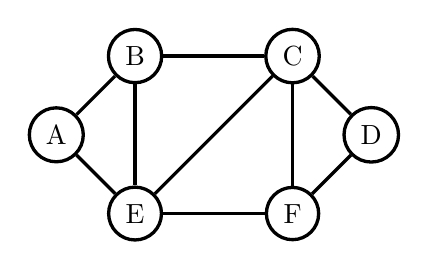
\begin{tikzpicture}[scale=0.5]
  \node[draw,circle, very thick] (A) at (0,2) {A};
  \node[draw,circle, very thick] (B) at (2,4) {B};
  \node[draw,circle, very thick] (C) at (6,4) {C};
  \node[draw,circle, very thick] (D) at (8,2) {D};
  \node[draw,circle, very thick] (E) at (2,0) {E};
  \node[draw,circle, very thick] (F) at (6,0) {F};
  \draw[very thick] (A) -- (B);
  \draw[very thick] (A) -- (E);
  \draw[very thick] (B) -- (C);
  \draw[very thick] (B) -- (E);
  \draw[very thick] (C) -- (D);
  \draw[very thick] (C) -- (E);
  \draw[very thick] (C) -- (F);
  \draw[very thick] (D) -- (F);
  \draw[very thick] (E) -- (F);
\end{tikzpicture}
